\documentclass[tikz,border=10pt]{standalone}
\usepackage{tikz}
\usetikzlibrary{arrows.meta,patterns,positioning}

\begin{document}
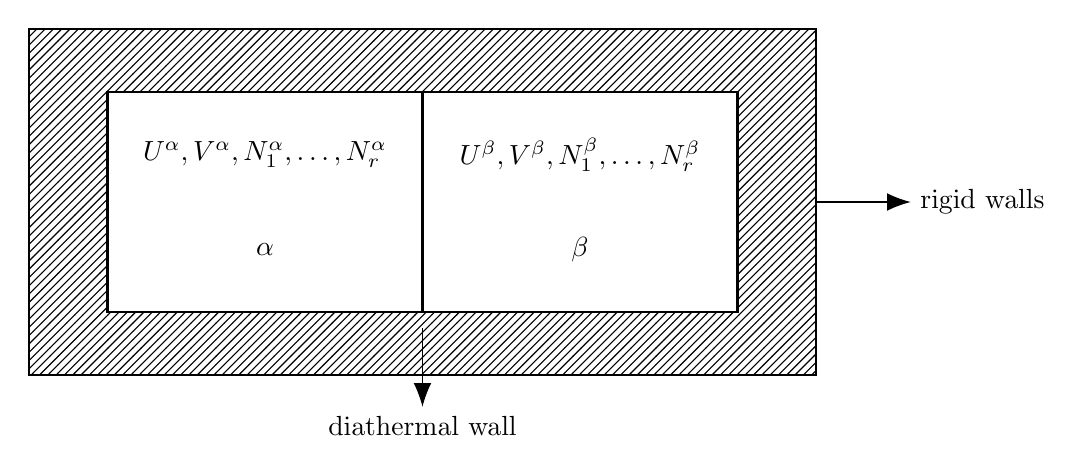
\begin{tikzpicture}
    % Outer rigid walls
    \draw[thick,pattern=north east lines] (-5,-2.2) rectangle (5,2.2);
    % Inner system box
    \draw[thick,fill=white] (-4,-1.4) rectangle (4,1.4);
    % Diathermal wall
    \draw[very thick] (0,-1.4) -- (0,1.4);

    % Left and right labels
    \node at (-2,0.6) {$U^\alpha, V^\alpha, N_1^\alpha,\ldots,N_r^\alpha$};
    \node at (2,0.6) {$U^\beta, V^\beta, N_1^\beta,\ldots,N_r^\beta$};
    \node at (-2,-0.6) {$\alpha$};
    \node at (2,-0.6) {$\beta$};

    % Labels
    \draw[-{Latex[length=3mm]}] (0,-1.6) -- (0,-2.6) node[below] {diathermal wall};
    \draw[-{Latex[length=3mm]}] (5,0) -- (6.2,0) node[right] {rigid walls};
\end{tikzpicture}
\end{document}
